\documentclass[]{article}
\usepackage[pdftex,paperwidth=434pt,paperheight=235pt,noheadfoot,left=0pt,top=0pt]{geometry}
\usepackage{graphicx}

\begin{document}
\noindent
%\scalebox{0.8819}[0.8966]{
\begin{picture}(432,234)
\put(-108,-158){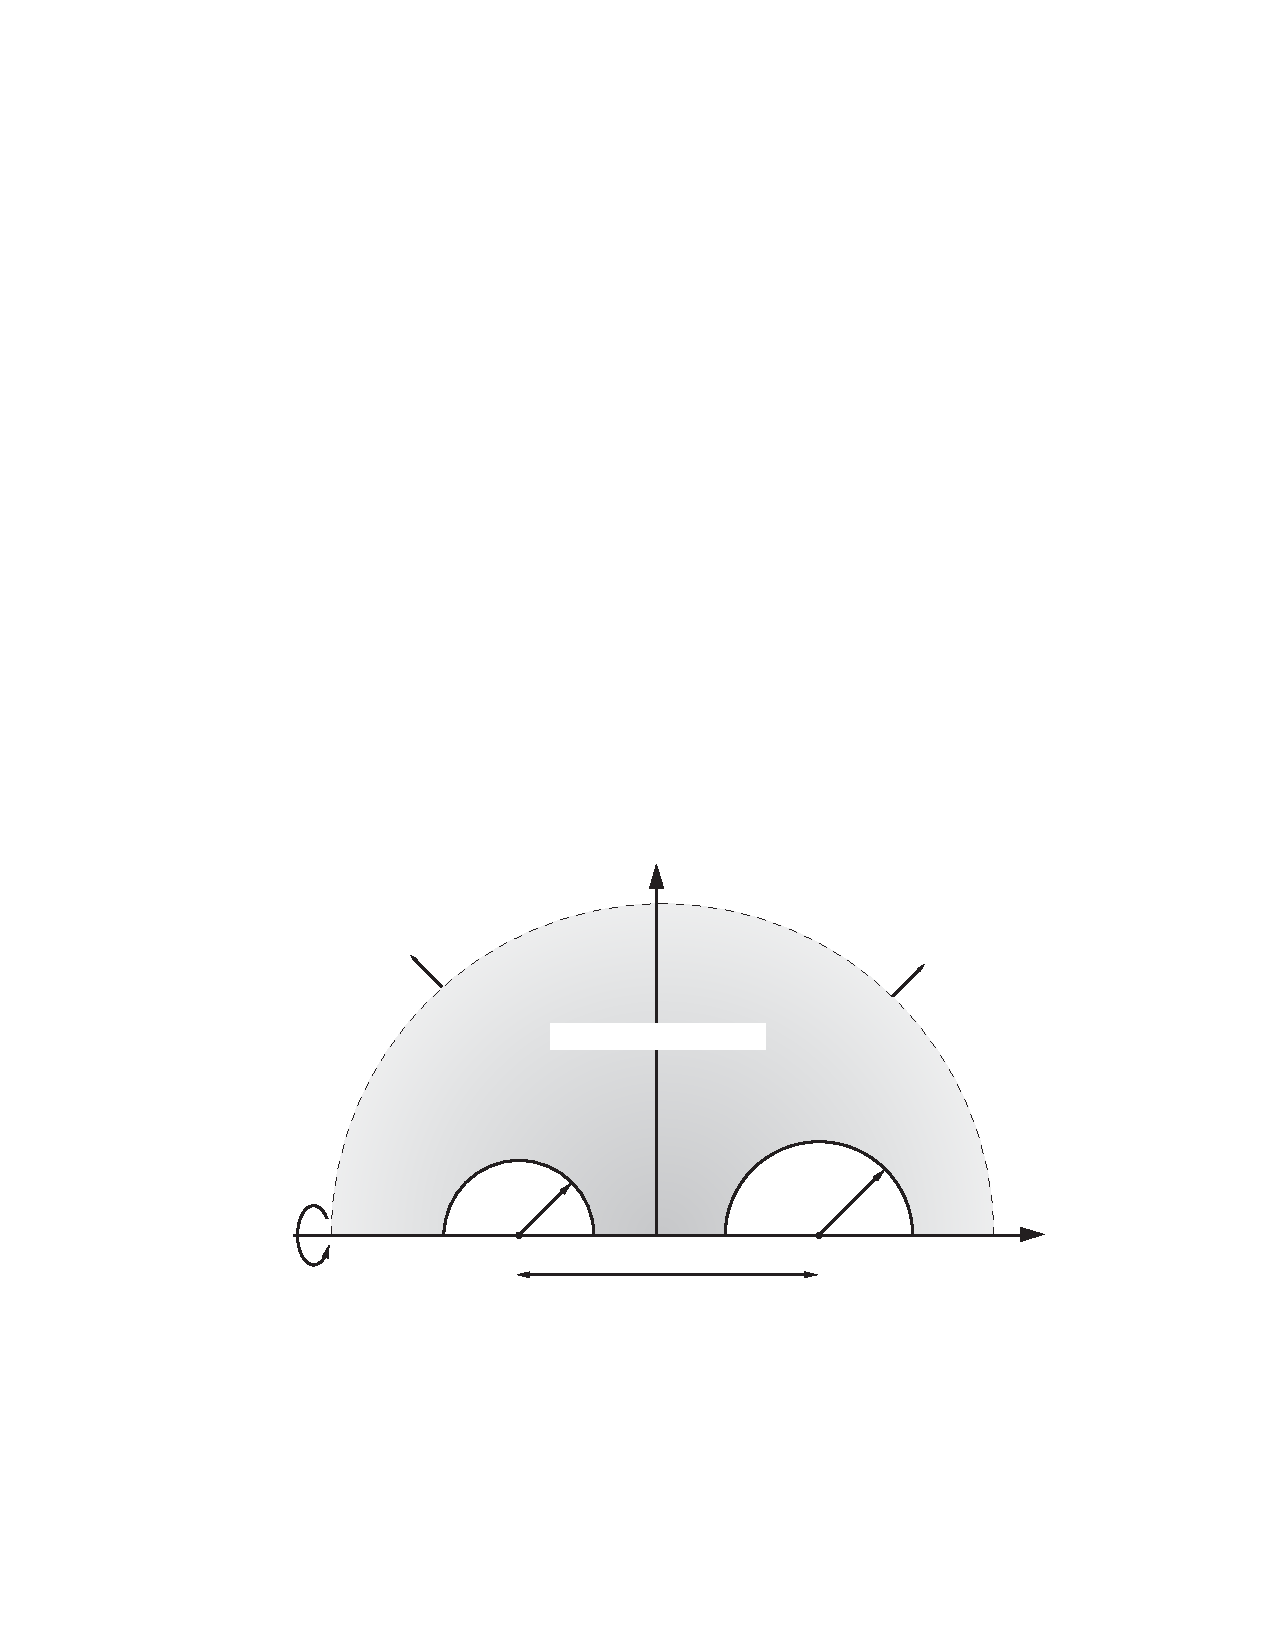
\includegraphics[width=8.5in]{PDFnotext/Figure9_1.pdf}}
\put(212,218){$\rho$}
\put(395,40){$z$}
\put(54,25){$\phi$}
\put(208,12){$\beta$}
\put(281,29){$\zeta_1$}
\put(138,29){$\zeta_2$}
\put(300,62){$1$}
\put(143,62){$1/\alpha$}
\put(82,178){$\infty$}
\put(336,173){$\infty$}
\put(157,134){Computational Domain}
\end{picture}
%}
\end{document}
